\section{\textit{\textbf{Elasticsearch}}}
\textit{\textbf{Elasticsearch}} je besplatan, distribuirani, otvoreni alat za skladištenje, pretragu i analizu \textit{(eng. search and analytics engine)}, raznih tipova podataka, uključujući tekstualne, numeričke, geo-prostorne \textit{(eng. geospatial)}, strukturne i nestrukturne \cite{elastic-elasticsearch}. Manipulacija podataka je ostvarena \textit{REST API}-jem, a alat omogućava izvanrednu horizontalnu skalabilnost. \textit{\textbf{Elasticsearch}} je zasnovan na \textbf{\textit{Apache Lucene} biblioteci} \cite{apache-lucene}, tj. ideji indeksiranja podataka na osnovu samog sadržaja. Podaci se skladište kao dokumenti, koji pripadaju jednom indeksu, dok je uz pomoć distribuiranog modela, indekse moguće podeliti na manje komponente, odnosno krhotine \textit{(eng. shard)}, koji mogu biti rasprostranjeni kroz veći broj čvorova \textit{(eng. node)}. Trenutno aktuelna verzija na kojoj se zasniva opis alata jeste verzija 8.6.

\subsection{Osnove \textit{\textbf{Elasticsearch}}-a}\label{subsection:osnove-elasticsearch-a}
\textit{\textbf{Elasticsearch}} arhitektura je projektovana za prikupljanje dokumenata, koji se skladište kao \textit{JSON} objekti \cite{json}. Alat podržava ugnježdene strukture, što olakšava obradu kompleksnih podataka i upita. Za praćenje informacija o dokumentima dodeljuju se specijalni atributi, odnosno meta-podaci, koji počinju donjom crtom. Važni meta-podaci su:
\begin{itemize}
    \item \textbf{\_index} – predstavlja kom indeksu dokument pripada. U analogiji, npr. sa relacionim bazama, ovo bi predstavljalo jednu bazu podataka.
    \item \textbf{\_type} – predstavlja klasu, odnosno mapiranje koje bi trebalo da ima svaki dokument koji pripada istom tipu. Ovo je analogno tabeli u relacionim bazama podataka. Trenutna verzija alata ovo polje tretira kao zastarelo \textit{(eng. deprecated)}, ostavljeno je samo radi kompatibilnosti sa starijim verzijama alata.
    \item \textbf{\_id} – jedinstveni identifikator dokumenta u okviru tipa.
    \item \textbf{\_version} – predstavlja broj izmena dokumenta, odnosno koliko puta je dokument bio kreiran, ažuriran, obrisan.
\end{itemize}

\par
Glavni elementi arhitekture \textit{\textbf{Elasticseach}}-a su: \textbf{klaster}, \textbf{čvor}, \textbf{krhotina} i \textbf{analizator}, čija je organizacija predstavljena na slici \ref{diagram:ahritektura-elasticsearch-alata}.

\begin{figure}[H]
    \centering
    \fboxsep=0.025\columnwidth%padding thickness
    \fboxrule=1pt%border thickness
    \fbox{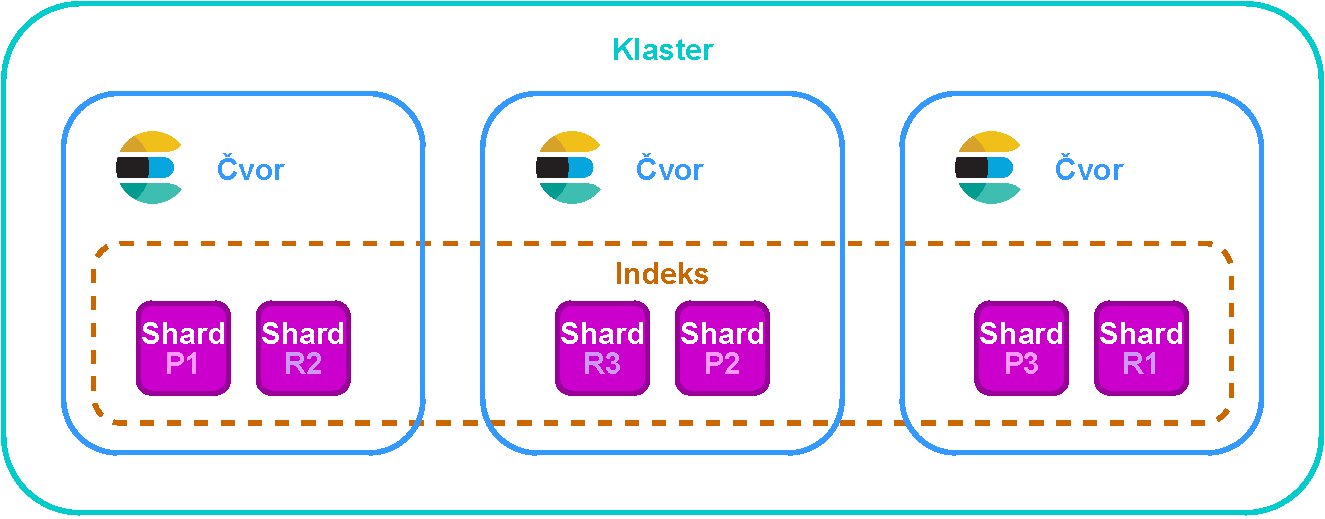
\includegraphics[width=0.95\columnwidth]{images/Elasticsearch-architecture.pdf}}
    \caption{\textit{Arhitektura \textbf{Elasticsearch} alata}}
    \label{diagram:ahritektura-elasticsearch-alata}
\end{figure}

\par
\textbf{Klaster} predstavlja grupu čvorova koji skladište podatke. U okviru konfiguracionog fajla \textit{\textbf{config/Elasticsearch.yml}} \footnote{\textit{YAML} format je dostupan u okviru \cite{YAML}} se može precizirati broj čvorova koji bivaju startovani u klasteru, kao i fizička ili virtualna adresa svakog od čvorova. Čvorovi u okviru jednog klastera su logički povezani i mogu razmenjivati podatke jedni sa drugima. Pri pokretanju, sistem automatski kreira jedan klaster sa jednim čvorom u njemu, što je dovoljno za osnovne potrebe prosečnog korisnika.

\par
\textbf{Čvor} ne predstavlja server, već jednu instancu \textit{\textbf{Elasticsearch}}-a, odnosno proces. Svaka instanca pripada jednom klasteru i zajedno, sa ostalim čvorovima u klasteru radi na rešavanju istog zadatka. Svaki čvor se može konfigurisati tako da obavlja barem jednu, a može obavljati više uloga u klasteru. Uloge koje čvoru mogu biti dodeljene obuhvataju:
\begin{itemize}
\item \textbf{Master čvor} – vrši kontrolu nad klasterom u vidu koordinacije čvorova koji pripadaju klasteru. Ovi čvorovi su odgovorni za operacije nad klasterom \textit{(eng. clasterwide operations)}, poput kreiranja i brisanja indeksa.
\item \textbf{Data čvor} – vrši skladištenje i odgovoran je za invertovani indeks podataka. Ovo je podrazumevana uloga čvora.
\item \textbf{Klijentski čvor} – predstavlja raspoređivač opterećenja \textit{(eng. load balancer)}\cite{Sanders2019-hv} koji vrši usmeravanje pristiglih zahteva različitim čvorovima u klasteru.
\end{itemize}

\par
Za ostvarivanje komunikacije se koriste dva glavna porta:
\begin{itemize}
    \item \textbf{Port 9200} – koristi se za filtriranje zahteva koji dolaze izvan klastera. Ovo su zahtevi \textit{REST API}-ja koji se koriste za izvršavanje upita, indeksiranje i slično.
    \item \textbf{Port 9300} – koristi se za među-čvornu \textit{(eng. inter-node)} komunikaciju.
\end{itemize}

\par
\textbf{Krhotina} predstavlja podskup dokumenata u okviru jednog indeksa. Naime, indeks nema ograničen broj dokumenata, niti ograničen memorijski kapacitet koji može da skladišti. Ukoliko se desi prekoračenje memorije na jednom od čvorova, \textit{\textbf{Elasticsearch}} prestaje sa radom i javlja grešku. Kako bi se ovaj problem rešio, indeksi se dele na krhotine, koje označavaju skalabilnu jedinicu za indeksiranje i omogućavaju distribuciju jednog indeksa na više čvorova. Ovim se postiže horizontalna skalabilnost sistema. Svaka krhotina funkcioniše kao nezavisan \textit{Lucene} indeks \cite{apache-lucene}, koji može biti skladišten bilo gde u klasteru.

\par
\textbf{Replika} predstavlja kopiju krhotine indeksa, dok se originalna krhotina naziva primarnom \textit{(eng. primary shard)}. Redundantnost podataka je glavni mehanizam na koji se sistemi otporni na greške oslanjaju \cite{Sanders2019-hv}. S obzirom da se radi o distribuiranom sistemom, ukoliko bi neki od čvorova otkazao, krhotine indeksa koje sadrži bi bile nedostupne, a samim tim i svi dokumenti koji se nalaze u nedostupnim podskupovima. Iz tog razloga se formiraju replike i dodeljuju različitim čvorovima u sistemu. Pored otpornosti na otkaze, ovo omogućava i brže pretraživanje podataka, jer više čvorova koji sadrže istu kopiju krhotine indeksa mogu istovremeno da vrše njenu pretragu i time ubrzaju proces pretrage indeksa u celini. Broj replika nije ograničen i mogu se precizirati nakon kreiranja indeksa, međutim, treba voditi računa jer iako je ovim čitanje ubrzano, svaka modifikacija je time znatno složenija.

\par
\textbf{Analizatori} imaju zadatak da vrše parsiranje fraza i izraza u konzistentne termine. Ovo se odvija u procesu indeksiranja. Svaki analizator je sačinjen od jednog tokenizatora \textit{(eng. tokenizer)} \footnote{Tokenizacija je proces razgraničenja i moguće klasifikacije delova niza ulaznih znakova. Dobijeni tokeni se zatim prosleđuju nekom drugom obliku obrade. Proces se može smatrati podzadatkom raščlanjivanja ulaza.\cite{tokenization}} i većeg broja filtera tokena. Kada se naiđe na određeni izraz, tokenizator može da podeli izraz u prethodno definisane termine. U ovome se krije još jedna tajna brze pretrage podataka.
